Nel Frontend\G{} è stato utilizzato il pattern architetturale Model-View-Presenter (MVP), design diffuso nelle WebApp, con lo scopo di separare le componenti di
visualizzazione dalla loro implementazione.
Il pattern si suddivide in tre elementi:
\begin{itemize}
    \item Model: elemento dove sono definiti i dati
    \item View: elemento passivo per la visualizzazione dei dati
    \item Presenter: elemento che fa da mediatore tra la View e il Model tramite data-binding ed eventi, prelevando o modificando dati del Model 
\end{itemize}
Quando l'utente interagisce con l'applicazione, la parte di View è incaricata di visualizzare i dati 
e di notificare le azioni dell'utente, la parte del Presenter fa da tramite per le interazioni tra View e Model, prelevando i dati da quest'ultimo e visualizzandoli, 
oltre che a rispondere in modo corretto agli eventi sollevati dalla View, modificando i dati del Model di conseguenza.
Il Model si occupa della persistenza dei dati oltre che a essere in grado di ottenerli tramite delle chiamate API\G{} (tramite metodo POST o GET) che si occuperà di interfacciarsi con
il Backend\G, il quale restituirà i dati o gli errori risultati dalla chiamata. 

A causa della scelta del framework\G{} Svelte\G{} la View non è una classe perchè è un Componente Svelte, 
che si compone da un blocco di script, un blocco di HTML\G{} ed un blocco di stile.
Lo script viene utilizzato soltanto per inizializzare il Presenter, per il resto la View è passiva come previsto dal pattern MVP. 

La reattività ai cambiamenti dei dati del Model (e anche nel Presenter) non è implementata con una pattern Observer standard,
bensì a livello del singolo campo all'interno dei Model con un tipo speciale `Writable' che può essere osservato tramite il metodo subscribe.

\begin{figure}[!h]
    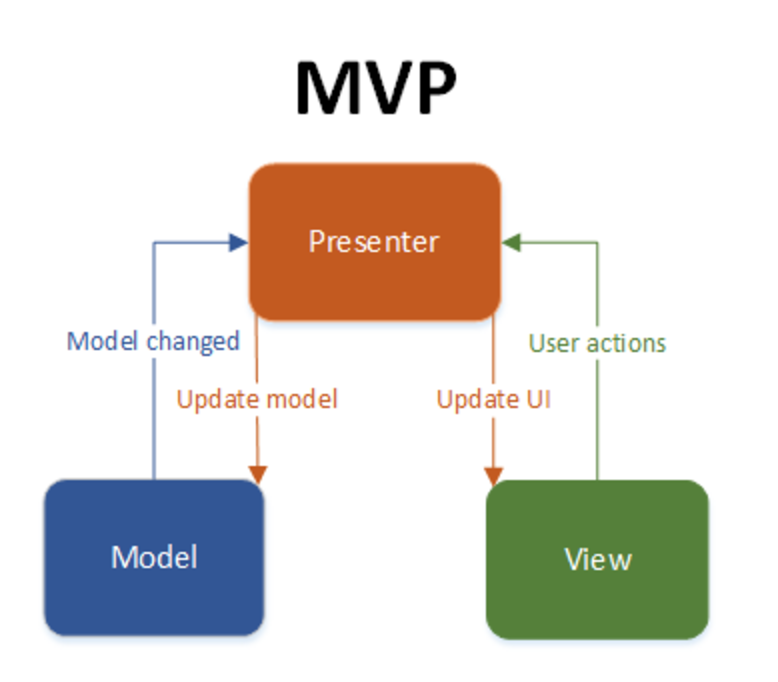
\includegraphics[width=10cm]{sezioni/images/mvp.png}
    \centering
    \caption{Schema pattern MVP}
\end{figure}

I punti di forza individuati in questo pattern sono che ogni classe Presenter possa gestire 
una classe View alla volta, quindi l'esistenza di una relazione uno a uno e questo permette di avere maggiore 
controllo sulle varie componenti, e la netta separazione presente tra Model e View. 
Quest'ultima risulta un punto chiave perchè permette di facilitare il testing relativo ai Presenter.

\subsection{Diagramma delle classi}
\begin{figure}[!h]
    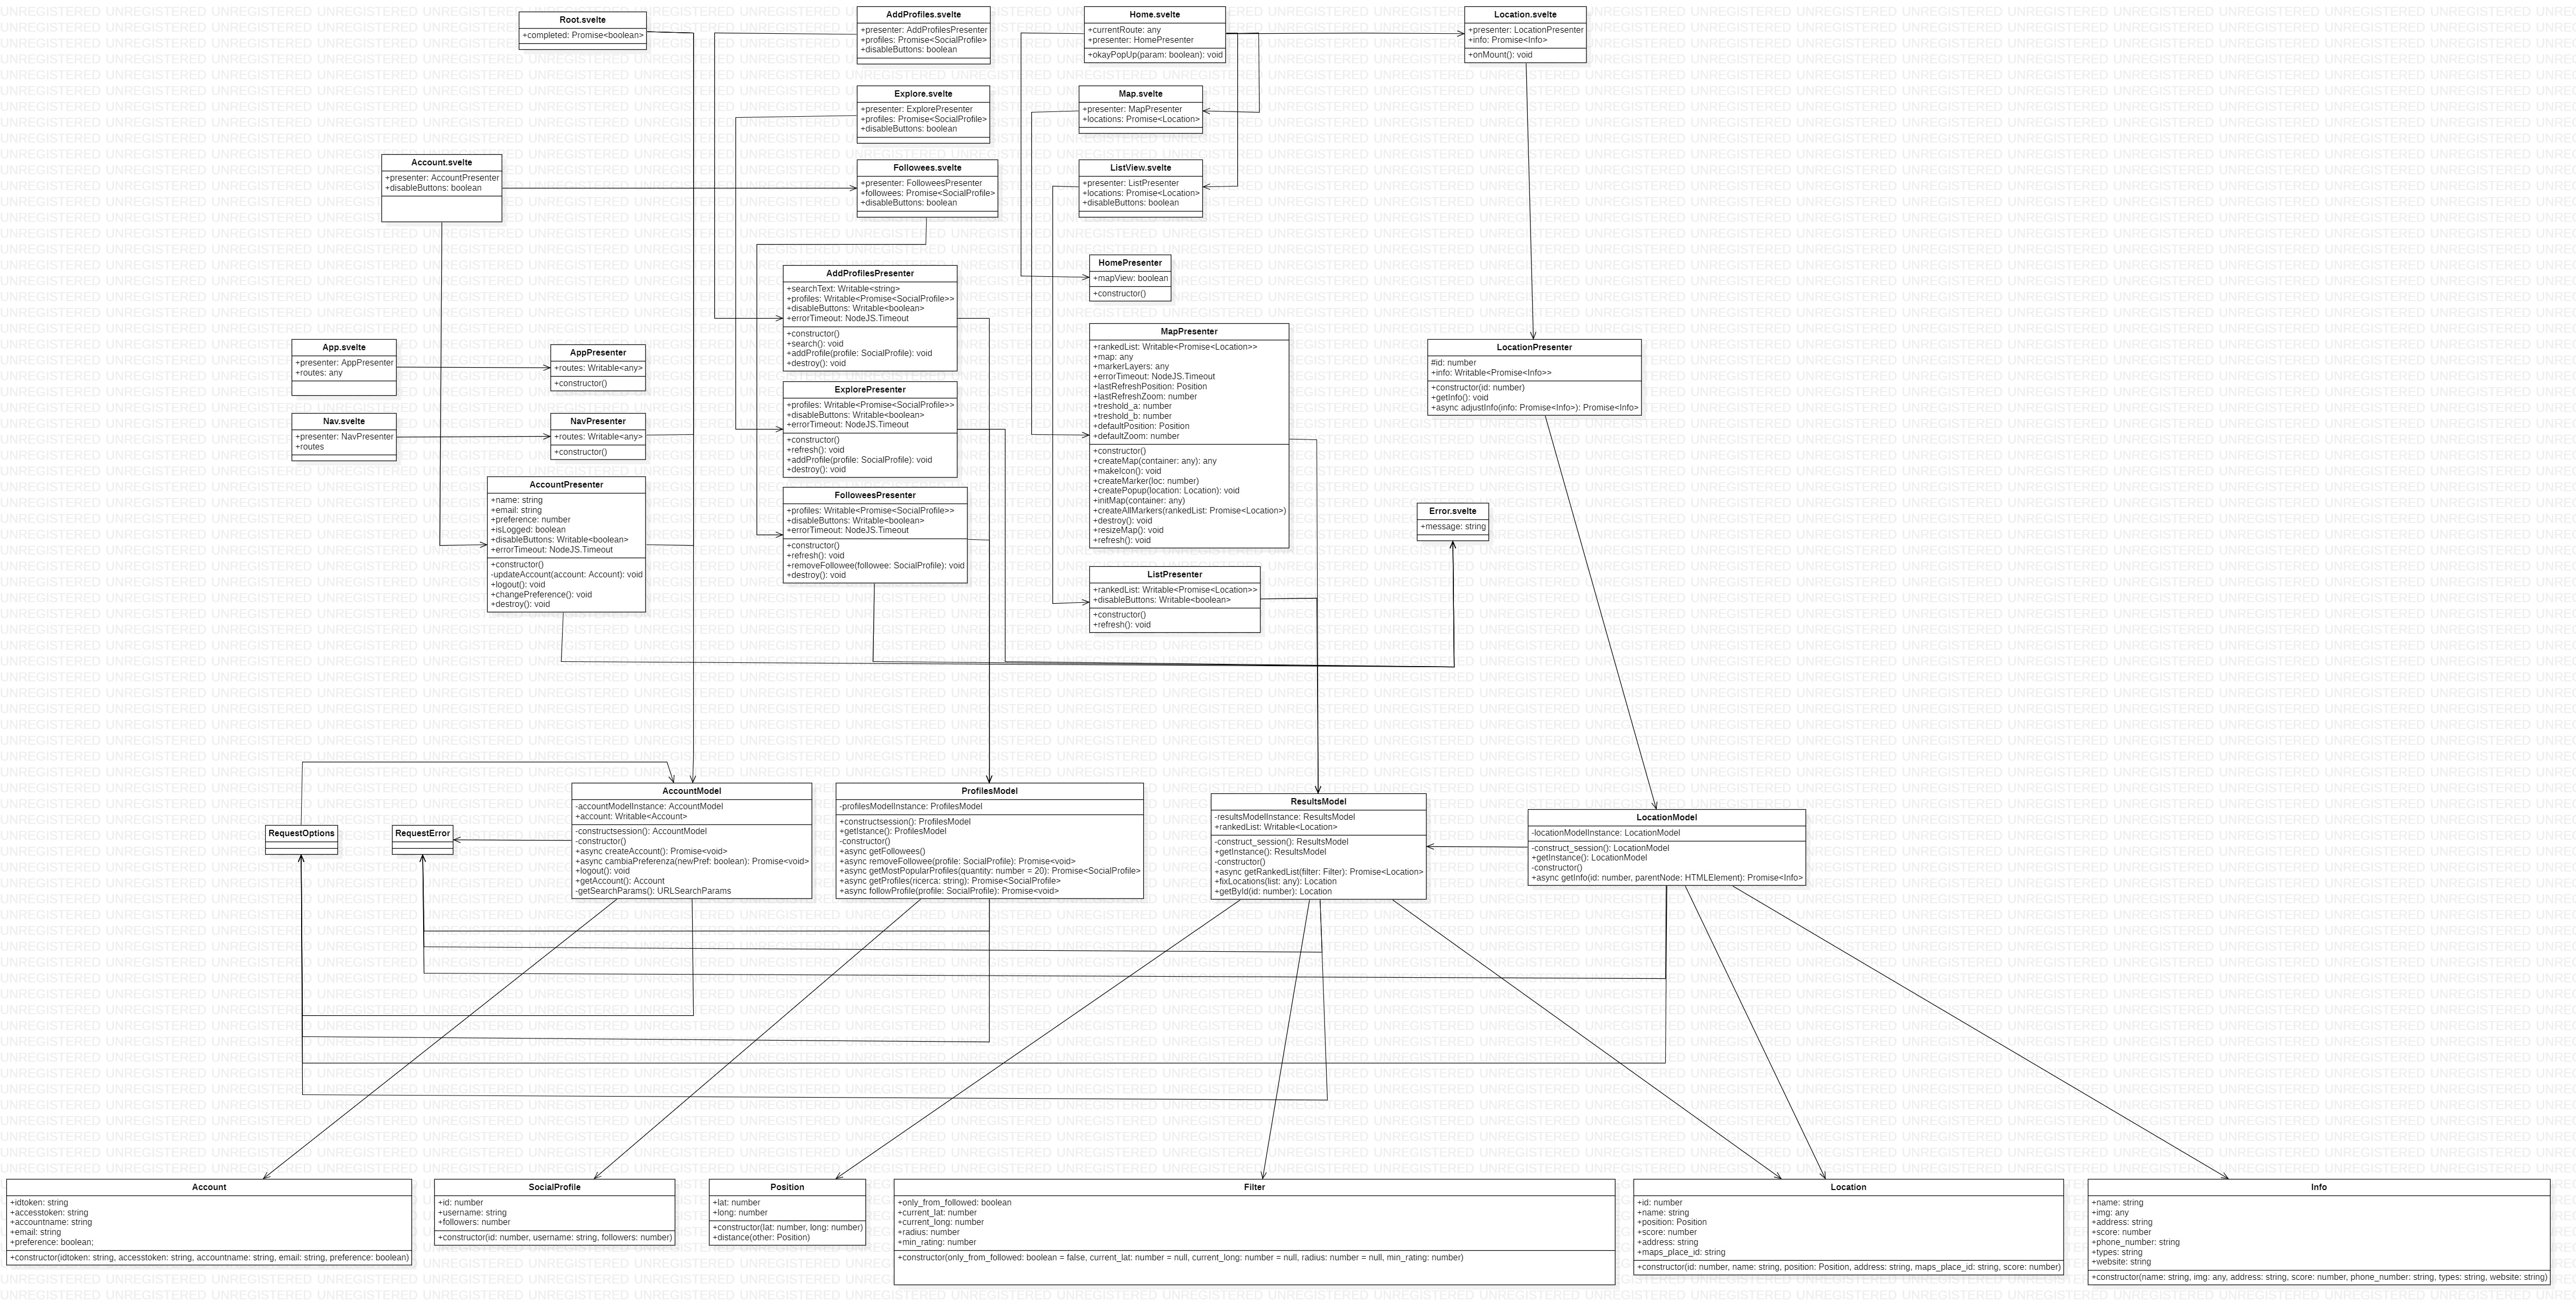
\includegraphics[width=16cm]{sezioni/images/Main.jpg}
    \centering
    \caption{Frontend - Diagramma delle classi}
\end{figure}

\subsection{Descrizione delle classi}
    \subsubsection{Models}
        I Models si occupano della persistenza dei dati e dell'interfacciamento con le varie API usate. Utilizzano la pattern singleton per la creazione di un istanza, e assieme alla creazione viene anche controllato il SessionStorage 
        per dati utili all'inizializzazione di un certo Model, sintomo di dati fondamentali che vanno mantenuti in memoria anche a seguito del cambio di pagina. Inoltre, mettono a disposizione alcuni membri Writable a cui ci si può iscrivere per ricevere i cambiamenti.
        Tutti i Model contengono codice asincrono che viene gestito tramite il sistema nativo delle Promsse Javascript (inclusa la sintassi async/await).
        \begin{itemize}
            \item AccountModel: Si occupa delle funzionalità di login, come decifrare i token ritornati dal login gestito da AWS Cognito\G{} per ottenere le informazioni sull'account. Si occupa delle funzionalità di gestione dell'account oltre a renderlo disponibile alle altre parti dell'applicazione.
            \item ResultsModel: Si occupa della gestione delle liste dei Luoghi da visualizzare all'interno dell'applicazione.
            \item ProfilesModel: Si occupa delle funzionalità legate ai profili social, per esempio seguire o rimuovere dai seguiti un profilo, oppure ottenere le liste dei profili seguiti o più popolari.
            \item LocationModel: Si occupa della fornitura delle informazioni dettagliate legate ad un singolo Luogo, interfacciandosi con la Maps API di Google per ottenere tali informazioni.
            \item RequestOptions: Si occupa della formattazione corretta delle opzioni di richiesta all'API, in modo da aderire alla specifica API.
        \end{itemize}
    \subsubsection{Presenters}
        I Presenters in generale si occupano di collezionare dati dai vari Model di bisogno e contenerli nella formattazione corretta per la visualizzazione diretta all'interno delle View, essi presentano molti membri Writable che consentono
        un'integrazione molto naturale con le View in quanto un membro di questo tipo visualizzato si aggiorna automaticamente in seguito ai cambiamenti. I Presenter sono attenti a sottoscriversi ai cambiamenti dei Model quando necessario per mostrare dati sempre aggiornati e rilevanti.
    \subsubsection{View}
        Le View sono dei componenti bene o male passivi, in quanto il codice scritto si limita alla delegazione degli eventi verso il Presenter, ed alla visualizzazione di dati statici o dinamici (tipo Writable). 
        Questi file vengono compilati automaticamente dalla libreria Svelte per diventare delle View funzionali e responsive ai cambiamenti.

